Supongamos que un largo conjunto de funciones lineales de la forma $y = m_ix + b_i$ es dado junto
con un largo número de pregunta. Cada pregunta consiste de un valor $x$ y pregunta por el mínimo valor
que puede ser obtenido si seleccionamos una de las funciones lineales y se evalúa en $x$. Por ejemplo,
supongamos que nuestras funciones son $y = 4$, $y = \frac{4}{3} + \frac{3}{2}x $, $y=12x-3$, 
$y=3-\frac{1}{2}$ y recibimos la pregunta $x = 1$. Necesitamos identificar cual de esas funciones tiene el 
menor valor de y para $x = 1$, o cual es ese valor. (Es la función $y = \frac{4}{3} + \frac{3}{2}x $ tiene 
un valor de 2). Ver la imagen de abajo.

% TODO: \usepackage{graphicx} required
\begin{figure*}[h!]
	\centering
	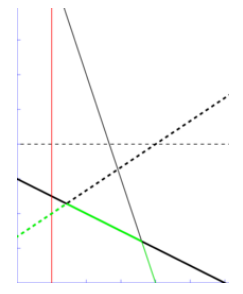
\includegraphics[width=0.30\linewidth]{img/convex_hull_trick}

	\label{fig:convexhulltrick}
\end{figure*}


El truco de la envoltura convexa (\emph{convex hull trick}) es una técnica (posiblemente mejor clasificado como una estructura de datos) usada para determinar eficientemente, después de un procesamiento, cuales miembros de un conjunto de funciones lineales de una variable alcanzan un valor extremo para un valor dado de la variable independiente. 